%\documentclass[journal,onecolumn]{IEEEtran}
\documentclass[11pt, oneside]{article}  
\usepackage{geometry}    
\geometry{letterpaper,margin=1in}       

\usepackage{amsmath} % special symbols
\usepackage{amssymb} % more special symbols
\usepackage{epsfig} % needed for including figures
\usepackage{lipsum} % generate placeholder text
\usepackage[hyphens]{url} % line break URLs
\usepackage[usenames,dvipsnames,svgnames,table]{xcolor} % custom color definition
\usepackage[figure]{algorithm2e} % advanced written algorithm handling
\usepackage{graphicx} % advanced graphic manipulation handling
\usepackage{epstopdf} % converts vector graphics (eps) to pdf for embedding
\usepackage{longtable} % allows tables to break across multiple pages
\usepackage{makeidx} % create an index
\usepackage{framed}
\usepackage{placeins}
\usepackage{enumerate}
\usepackage{cite}
\usepackage[T1]{fontenc}
\usepackage[utf8]{inputenc}
\usepackage{tabularx,ragged2e,booktabs,caption}
\newcolumntype{C}[1]{>{\Centering}m{#1}}
\renewcommand\tabularxcolumn[1]{C{#1}}


% *** SUBFIGURE PACKAGES ***
%\ifCLASSOPTIONcompsoc
%  \usepackage[caption=false,font=normalsize,labelfont=sf,textfont=sf]{subfig}
%\else
%  \usepackage[caption=false,font=footnotesize]{subfig}
%\fi
% subfig.sty, written by Steven Douglas Cochran, is the modern replacement
% for subfigure.sty, the latter of which is no longer maintained and is
% incompatible with some LaTeX packages including fixltx2e. However,
% subfig.sty requires and automatically loads Axel Sommerfeldt's caption.sty
% which will override IEEEtran.cls' handling of captions and this will result
% in non-IEEE style figure/table captions. To prevent this problem, be sure
% and invoke subfig.sty's "caption=false" package option (available since
% subfig.sty version 1.3, 2005/06/28) as this is will preserve IEEEtran.cls
% handling of captions.
% Note that the Computer Society format requires a larger sans serif font
% than the serif footnote size font used in traditional IEEE formatting
% and thus the need to invoke different subfig.sty package options depending
% on whether compsoc mode has been enabled.
%
% The latest version and documentation of subfig.sty can be obtained at:
% http://www.ctan.org/pkg/subfig




% *** FLOAT PACKAGES ***
%
%\usepackage{fixltx2e}
% fixltx2e, the successor to the earlier fix2col.sty, was written by
% Frank Mittelbach and David Carlisle. This package corrects a few problems
% in the LaTeX2e kernel, the most notable of which is that in current
% LaTeX2e releases, the ordering of single and double column floats is not
% guaranteed to be preserved. Thus, an unpatched LaTeX2e can allow a
% single column figure to be placed prior to an earlier double column
% figure.
% Be aware that LaTeX2e kernels dated 2015 and later have fixltx2e.sty's
% corrections already built into the system in which case a warning will
% be issued if an attempt is made to load fixltx2e.sty as it is no longer
% needed.
% The latest version and documentation can be found at:
% http://www.ctan.org/pkg/fixltx2e


%\usepackage{stfloats}
% stfloats.sty was written by Sigitas Tolusis. This package gives LaTeX2e
% the ability to do double column floats at the bottom of the page as well
% as the top. (e.g., "\begin{figure*}[!b]" is not normally possible in
% LaTeX2e). It also provides a command:
%\fnbelowfloat
% to enable the placement of footnotes below bottom floats (the standard
% LaTeX2e kernel puts them above bottom floats). This is an invasive package
% which rewrites many portions of the LaTeX2e float routines. It may not work
% with other packages that modify the LaTeX2e float routines. The latest
% version and documentation can be obtained at:
% http://www.ctan.org/pkg/stfloats
% Do not use the stfloats baselinefloat ability as the IEEE does not allow
% \baselineskip to stretch. Authors submitting work to the IEEE should note
% that the IEEE rarely uses double column equations and that authors should try
% to avoid such use. Do not be tempted to use the cuted.sty or midfloat.sty
% packages (also by Sigitas Tolusis) as the IEEE does not format its papers in
% such ways.
% Do not attempt to use stfloats with fixltx2e as they are incompatible.
% Instead, use Morten Hogholm'a dblfloatfix which combines the features
% of both fixltx2e and stfloats:
%
% \usepackage{dblfloatfix}
% The latest version can be found at:
% http://www.ctan.org/pkg/dblfloatfix




% *** PDF, URL AND HYPERLINK PACKAGES ***
%
%\usepackage{url}
% url.sty was written by Donald Arseneau. It provides better support for
% handling and breaking URLs. url.sty is already installed on most LaTeX
% systems. The latest version and documentation can be obtained at:
% http://www.ctan.org/pkg/url
% Basically, \url{my_url_here}.




% *** Do not adjust lengths that control margins, column widths, etc. ***
% *** Do not use packages that alter fonts (such as pslatex).         ***
% There should be no need to do such things with IEEEtran.cls V1.6 and later.
% (Unless specifically asked to do so by the journal or conference you plan
% to submit to, of course. )


% correct bad hyphenation here
\hyphenation{op-tical net-works semi-conduc-tor}


\newcommand{\TODO}[1]{\textcolor{red}{\textbf{TODO: } #1}}



\begin{document}

\title{Identification of Conserved Regions\\ in CRISPR protein family}

% make the title area
\maketitle

\begin{center}
\begin{tabular}{ c c c }
 Christine Baek & Qi Chu & Yanyu Liang \\ 
christib@andrew.cmu.edu & qchu@andrew.cmu.edu & yanyul@andrew.cmu.edu \\     
\end{tabular}\\
\smallskip
\smallskip
Computational Biology, Carnegie Mellon University
\end{center}

\bigskip

% As a general rule, do not put math, special symbols or citations
% in the abstract
\begin{abstract}
The abstract goes here.
\end{abstract}

% no keywords





\section{Introduction}

\TODO{Christine : brief intro}

\subsection{CRISPR/Cas} 
\TODO{Christine writes about CRISPR bg}
Subsection text here.

\subsection{Past Approaches}
\TODO{Qi : summarize the HMMer approach?}

\subsection{Approaches in This Paper}
\TODO{everyone?}

\subsection{Goal of Paper}
\TODO{Yanyu : short discussion of our goal in this paper}


% An example of a floating figure using the graphicx package.
% Note that \label must occur AFTER (or within) \caption.
% For figures, \caption should occur after the \includegraphics.
% Note that IEEEtran v1.7 and later has special internal code that
% is designed to preserve the operation of \label within \caption
% even when the captionsoff option is in effect. However, because
% of issues like this, it may be the safest practice to put all your
% \label just after \caption rather than within \caption{}.
%
% Reminder: the "draftcls" or "draftclsnofoot", not "draft", class
% option should be used if it is desired that the figures are to be
% displayed while in draft mode.
%
%\begin{figure}[!t]
%\centering
%\includegraphics[width=2.5in]{myfigure}
% where an .eps filename suffix will be assumed under latex, 
% and a .pdf suffix will be assumed for pdflatex; or what has been declared
% via \DeclareGraphicsExtensions.
%\caption{Simulation results for the network.}
%\label{fig_sim}
%\end{figure}

% Note that the IEEE typically puts floats only at the top, even when this
% results in a large percentage of a column being occupied by floats.


% An example of a double column floating figure using two subfigures.
% (The subfig.sty package must be loaded for this to work.)
% The subfigure \label commands are set within each subfloat command,
% and the \label for the overall figure must come after \caption.
% \hfil is used as a separator to get equal spacing.
% Watch out that the combined width of all the subfigures on a 
% line do not exceed the text width or a line break will occur.
%
%\begin{figure*}[!t]
%\centering
%\subfloat[Case I]{\includegraphics[width=2.5in]{box}%
%\label{fig_first_case}}
%\hfil
%\subfloat[Case II]{\includegraphics[width=2.5in]{box}%
%\label{fig_second_case}}
%\caption{Simulation results for the network.}
%\label{fig_sim}
%\end{figure*}
%
% Note that often IEEE papers with subfigures do not employ subfigure
% captions (using the optional argument to \subfloat[]), but instead will
% reference/describe all of them (a), (b), etc., within the main caption.
% Be aware that for subfig.sty to generate the (a), (b), etc., subfigure
% labels, the optional argument to \subfloat must be present. If a
% subcaption is not desired, just leave its contents blank,
% e.g., \subfloat[].


% An example of a floating table. Note that, for IEEE style tables, the
% \caption command should come BEFORE the table and, given that table
% captions serve much like titles, are usually capitalized except for words
% such as a, an, and, as, at, but, by, for, in, nor, of, on, or, the, to
% and up, which are usually not capitalized unless they are the first or
% last word of the caption. Table text will default to \footnotesize as
% the IEEE normally uses this smaller font for tables.
% The \label must come after \caption as always.
%
%\begin{table}[!t]
%% increase table row spacing, adjust to taste
%\renewcommand{\arraystretch}{1.3}
% if using array.sty, it might be a good idea to tweak the value of
% \extrarowheight as needed to properly center the text within the cells
%\caption{An Example of a Table}
%\label{table_example}
%\centering
%% Some packages, such as MDW tools, offer better commands for making tables
%% than the plain LaTeX2e tabular which is used here.
%\begin{tabular}{|c||c|}
%\hline
%One & Two\\
%\hline
%Three & Four\\
%\hline
%\end{tabular}
%\end{table}


% Note that the IEEE does not put floats in the very first column
% - or typically anywhere on the first page for that matter. Also,
% in-text middle ("here") positioning is typically not used, but it
% is allowed and encouraged for Computer Society conferences (but
% not Computer Society journals). Most IEEE journals/conferences use
% top floats exclusively. 
% Note that, LaTeX2e, unlike IEEE journals/conferences, places
% footnotes above bottom floats. This can be corrected via the
% \fnbelowfloat command of the stfloats package.


\section{Methods}

All code and output files are available on \texttt{https://github.com/cookie223/CAS\_project}. 

Any reference to files in this report indicate filepath based on root of the repository. 

In this paper, we use 3 different approaches, each with different strengths and limits as for discovering patterns and information from multiple related sequences. Each method has its own section which discusses overview of algorithm/model, pros and cons of given model, detailed protocol and parameters, and analysis performed. 

Protein sequences were used (as opposed to DNA), to uncover preservation of \textit{Cas} protein's functional motifs. Protein sequence analysis much more appropriate for such purpose than DNA sequence especially for distantly related sequences. 

\subsection{Data Retrieval}

\TODO{Qi : talk about source of data}

\subsection{Sequence Alignment using Dynamic Programming} \label{dpProtocol}

Semiglobal ailgnment using Needleman-Wunsch\cite{needlemanwunsch} and Local Alignment using Smith-Waterman Algorithm\cite{smithwaterman} were implemented for pairwise sequence comparison.

code available at \texttt{https://github.com/cookie223/CAS\_project/tree/master/dp}

\medskip
\subsubsection{Model \& Algorithm Overview}

Semiglobal alignment and local alignment were performed on various \textit{Cas} sequences. Because certain families of \textit{Cas} proteins are composed of multiple genes, it is impossible to do a global alignment, or multiple sequence alignment with all \textit{Cas} sequences. Instead, \textit{s. pyogenes Cas9} was used as a reference sequence, to which all other \textit{Cas} sequence was aligned to in pairwise sequence alignment. 

\medskip
\subsubsection{Pros and Cons}

Because alignment were done against \textit{s. pyogenes Cas9} rather than a progressive alignment, for \textit{Cas} sequences highly divergent from \textit{s. pyogenes Cas9} may be aligned to an inaccurate site. Each alignment is guaranteed to return the global maximum or the most optimal alignment with given parameters, which may or may not be the actual corresponding motif. Also, this method assumes site independence, and does not discriminate conserved regions (which motifs would likely be part of) as opposed to fast-evolving regions.

\medskip
\subsubsection{Protocol} 
Following parameters were used for sequence alignment :
\begin{itemize}
\item Scoring Matrix = BLOSUM62 (BLASTP default)
\item Affine Gap Penalty = -10 (BLASTP default is 11)
\item Gap Extension Penalty = -1 (BLASTP default)
\item End Gap Penalty (for Semi-Global only) = -3
\end{itemize}

Gap opening / affine gap penalty was slightly lowered to relax requirement for opening gap, as this experiment is for identifying local regions rather than strict sequence search.

\medskip
\subsubsection{Analysis}

After each \textit{Cas} sequence was aligned to \textit{s. pyogenes Cas9}, it was then analyzed for the following values :
\begin{itemize}
\item Start position (row, col) of traceback
\item End position (row, col) of traceback
\item Alignment score (based on parameters discussed in section~\ref{dpProtocol}
\item Average Score per base : alignment score / number of bases in alignment
\item \% Sequence Aligned : length of alignment / length of query (non-reference) sequence
\end{itemize}

This was done for both semi-global and local alignment outputs. 

\bigskip
\subsection{Gibbs Sampling}
\medskip
\subsubsection{Model \& Algorithm Overview}
talk about overview of what the method does (method itself, not in detail of how you used it)

\medskip
\subsubsection{Pros and Cons}
of using the method - what is it capable of, what are the limitations ?

\medskip
\subsubsection{Protocol}
implementation details - justifications for decisions you made when you ran the experiment, parameters, etc.

\medskip
\subsubsection{Analysis}
Discuss METHOD for analysis, not the actual result/analysis itself. 

\bigskip
\subsection{Domain-specific profile HMM}
\medskip
\subsubsection{Model \& Algorithm Overview}
To find out whether a sequence of amino acid belongs some domain, we can build a model of the domain and try to match the sequence of the model. Profile Hidden Markov Model is one of the 
models we can build to figure out whether a sequence contains the domain. The model of profile HMM is shown in Figure \ref{HMM}. 

\begin{figure}[ht]
  \centering
  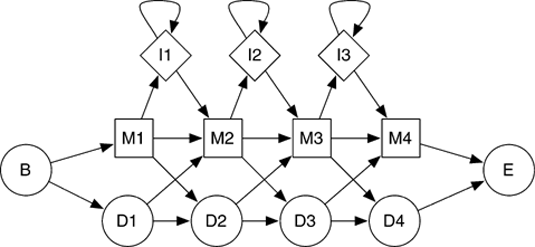
\includegraphics[scale = 0.7]{images/profileHMM}
      \caption{Profile Hidden Markov Model\cite{hmmer}}
      \label{HMM}
\end{figure}

\medskip
\subsubsection{Pros and Cons}
\begin{itemize}
\item Pros
\begin{enumerate}
\item We can leverage the abundant prior knowledge of Cas9 domain markers by building profile HMM using the alignment of the domains rather than the full sequence.
\item Compared with pair-wise sequence alignment, HMM can find more cases of distantly related sequences.
\item As shown in the figure, HMM can model insertions and deletions.
\end{enumerate}
\item Cons
\begin{enumerate}
\item To leverage the prior knowledge of domain markers, those markers need to be fetched separately from other data source rather than learned by the algorithm.
\item The number of parameters is very large and they need to be optimized.
\end{enumerate}
\end{itemize}

\medskip
\subsubsection{Protocol}
\begin{enumerate}[a.]
\item A set of \textit{Cas9} or \textit{Cas5} sequences and their domain markers are fetched from EMBL-EBI (http://www.ebi.ac.uk).
\item Sequences of each of the shared domains are subtracted from the full \textit{Cas9} or \textit{Cas5} sequences.
\item For each domain, multiple sequences from different \textit{Cas9} or \textit{Cas5} are aligned by Clustal Omega (http://www.clustal.org/).
\item  A profile HMM is built on the multiple sequence alignment for each domain by Hmmer (http://hmmer.org/)\cite{hmmer}.
\item Search for matches using the profile HMM in the sequences of all previously downloaded \textit{Cas} family proteins.
\end{enumerate}

\medskip
\subsubsection{Analysis}
For method testing, a set of globin sequences given in Hmmer\cite{hmmer} is used. Since there are \textit{Cas9} and \textit{Cas5} in the previously downloaded \textit{Cas} family proteins sequences, they also act as positive control since the method should be able to find the domains in these proteins.\\
For output analysis, HMM is able to give the probability of given sequence emitted from the underlying domain profile HMM.





\section{Results}

Each of the three approaches for identifying motifs of \textit{Cas} proteins and the resulting data are presented below. 


\subsection{Sequence Alignment using Dynamic Programming}

\begin{minipage}{\linewidth}
\smallskip
\centering
\captionof{table}{Semi-Global Alignment Output} \label{sgoutput} 
\begin{tabular}{ p{1.25in} C{.85in} *4{C{.75in}}}\toprule[1.5pt]
\bf Gene Name & \bf Alignment Score & \bf Average Score / base & \bf \% Sequence aligned & \bf Traceback Start & \bf Traceback End\\\midrule
Cas10\_Mtuberculosis & 234 & 0.212148685 & 1 & [1365][810] & [330][1]\\ 
Cas10\_Phorikoshii & 335 & 0.249813572 & 1 & [1368][762] & [41][1]\\ 
Cas10\_Ssolfataricus & 364 & 0.27063197 & 1 & [1322][1046] & [62][1]\\ 
Cas10\_Tvolcanium & 343 & 0.305976806 & 1 & [1203][776] & [146][1]\\ 
Cas1\_DvsH\_plasmid & 160 & 0.282186949 & 1 & [1297][344] & [734][1]\\ 
Cas1\_Gvaginalis & 163 & 0.332653061 & 1 & [1367][321] & [886][1]\\ 
Cas1\_K-12 & 105 & 0.243055556 & 0.911764706 & [428][306] & [1][28]\\ 
Cas1\_Tdenticola & 176 & 0.387665198 & 1 & [519][291] & [79][1]\\ 
Cas2\_K-12 & 65 & 0.5 & 1 & [528][95] & [400][1]\\ 
Cas2\_Lsalivarius & 64 & 0.444444444 & 1 & [617][102] & [476][1]\\ 
Cas2\_StB20-like & 68 & 0.586206897 & 1 & [217][88] & [102][1]\\ 
Cas3\_DvsH\_plasmid & 152 & 0.145315488 & 1 & [1059][703] & [32][1]\\ 
Cas3\_Gvaginalis & 260 & 0.229681979 & 0.858199753 & [1119][811] & [1][116]\\ 
Cas3\_K-12 & 233 & 0.185805423 & 1 & [1254][889] & [29][1]\\ 
Cas4\_K-12 & 171 & 0.341317365 & 1 & [1323][364] & [833][1]\\ 
Cas4\_Ssolfataricus & 87 & 0.294915254 & 1 & [679][203] & [387][1]\\ 
Cas4\_TtenaxKra & 57 & 0.230769231 & 1 & [573][191] & [330][1]\\ 
Cas5\_Gvaginalis & 140 & 0.309050773 & 1 & [1185][292] & [733][1]\\ 
Cas5\_K-12 & 79 & 0.302681992 & 0.8 & [261][225] & [1][46]\\ 
Cas6\_Cbotulinum & 158 & 0.478787879 & 1 & [740][230] & [414][1]\\ 
Cas6\_Hvolcanii\_plasmid & 99 & 0.25848564 & 1 & [1309][273] & [929][1]\\ 
Cas6\_Ssolfataricus & 118 & 0.280952381 & 1 & [1117][288] & [701][1]\\ 
Cas7\_Hvolcanii\_plasmid & 164 & 0.316602317 & 1 & [899][341] & [390][1]\\ 
Cas7\_K-12 & 171 & 0.341317365 & 1 & [1323][364] & [833][1]\\ 
Cas7\_Ssolfataricus & 147 & 0.267272727 & 1 & [950][312] & [404][1]\\ 
Cas8\_LsV & 136 & 0.265625 & 1 & [1289][314] & [783][1]\\ 
Cas8\_Pdistasois & 237 & 0.295511222 & 1 & [1342][573] & [559][1]\\ 
Cas8\_Pgingivalis & 212 & 0.280794702 & 1 & [1340][500] & [609][1]\\ 
Cas9\_Bthermosphacta & 1726 & 1.249818972 & 1 & [1365][1301] & [47][1]\\ 
Cas9\_Cindologenes & 476 & 0.282157676 & 1 & [1366][1444] & [3][1]\\ 
Cas9\_Cochracea & 375 & 0.276344878 & 0.650315347 & [1322][1427] & [1][500]\\ 
Cas9\_Hpullorum & 180 & 0.27820711 & 1 & [643][345] & [4][1]\\ 
Cas9\_Hpullorum\_2 & 330 & 0.391459075 & 1 & [1347][703] & [549][1]\\ 
Cas9\_Kkingae & 520 & 0.370634355 & 0.997172479 & [1341][1061] & [1][4]\\ 
Cas9\_Movipneumoniae & 519 & 0.340998686 & 0.988216811 & [1349][1273] & [1][16]\\ 
Cas9\_Nlactamica & 505 & 0.353889278 & 0.994459834 & [1368][1083] & [1][7]\\ 
Cas9\_Pacidlactici & 1786 & 1.209207854 & 0.999267399 & [1366][1365] & [1][2]\\ 
Cas9\_Pnultocida & 510 & 0.365068003 & 0.997161779 & [1348][1057] & [1][4]\\ 
Cas9\_Ranatipestifer & 391 & 0.239143731 & 1 & [1366][1406] & [3][1]\\ 
Cas9\_Sgallolyticus & 4529 & 3.274765004 & 0.999271137 & [1368][1372] & [1][2]\\ 
Cas9\_Smoniliformis & 514 & 0.327597196 & 1 & [1368][1260] & [3][1]\\ 
Cas9\_Spaucimobilis & 415 & 0.290616246 & 1 & [1362][1091] & [3][1]\\
\bottomrule[1.25pt]
\end {tabular}\par
\bigskip
Method as discussed in section~\ref{dpProtocol}. Visualization of data is available in Figure~\ref{dp1}
\end{minipage}

\begin{minipage}{\linewidth}
\smallskip
\centering
\captionof{table}{Local Alignment Output} \label{locoutput} 
\begin{tabular}{ p{1.25in} C{.85in} *4{C{.75in}}}\toprule[1.5pt]
\bf Gene Name & \bf Alignment Score & \bf Average Score / base & \bf \% Sequence aligned & \bf Traceback Start & \bf Traceback End\\\midrule
Cas10\_Mtuberculosis & 317 & 0.239064857 & 0.988888889 & [1345][808] & [46][8]\\ 
Cas10\_Phorikoshii & 313 & 0.246650906 & 0.874015748 & [1368][705] & [105][40]\\ 
Cas10\_Ssolfataricus & 432 & 0.316020483 & 0.864244742 & [1365][929] & [16][26]\\ 
Cas10\_Tvolcanium & 362 & 0.312878133 & 0.923969072 & [1312][749] & [165][33]\\ 
Cas1\_DvsH\_plasmid & 152 & 0.290630975 & 0.959302326 & [1237][342] & [728][13]\\ 
Cas1\_Gvaginalis & 120 & 0.270880361 & 0.99376947 & [1332][320] & [904][2]\\ 
Cas1\_K-12 & 107 & 0.29558011 & 0.666666667 & [1340][263] & [983][60]\\ 
Cas1\_Tdenticola & 124 & 0.294536817 & 0.965635739 & [1096][287] & [687][7]\\ 
Cas2\_K-12 & 43 & 0.651515152 & 0.663157895 & [1119][86] & [1055][24]\\ 
Cas2\_Lsalivarius & 77 & 0.611111111 & 0.794117647 & [621][101] & [496][21]\\ 
Cas2\_StB20-like & 72 & 1.028571429 & 0.568181818 & [738][87] & [669][38]\\ 
Cas3\_DvsH\_plasmid & 210 & 0.195712954 & 0.944523471 & [1099][683] & [48][20]\\ 
Cas3\_Gvaginalis & 261 & 0.244382022 & 0.937114673 & [1317][790] & [272][31]\\ 
Cas3\_K-12 & 248 & 0.245787909 & 0.750281215 & [1232][873] & [265][207]\\ 
Cas4\_K-12 & 177 & 0.353293413 & 0.848901099 & [1355][325] & [856][17]\\ 
Cas4\_Ssolfataricus & 100 & 0.304878049 & 0.827586207 & [1308][180] & [981][13]\\ 
Cas4\_TtenaxKra & 60 & 0.810810811 & 0.277486911 & [883][175] & [811][123]\\ 
Cas5\_Gvaginalis & 159 & 0.42513369 & 0.863013699 & [797][274] & [424][23]\\ 
Cas5\_K-12 & 77 & 0.292775665 & 0.68 & [493][184] & [233][32]\\ 
Cas6\_Cbotulinum & 132 & 0.371830986 & 0.82173913 & [453][215] & [99][27]\\ 
Cas6\_Hvolcanii\_plasmid & 93 & 0.322916667 & 0.648351648 & [755][225] & [468][49]\\ 
Cas6\_Ssolfataricus & 121 & 0.292978208 & 0.954861111 & [1208][286] & [799][12]\\ 
Cas7\_Hvolcanii\_plasmid & 177 & 0.5 & 0.692082111 & [416][297] & [63][62]\\ 
Cas7\_K-12 & 177 & 0.353293413 & 0.848901099 & [1355][325] & [856][17]\\ 
Cas7\_Ssolfataricus & 139 & 0.445512821 & 0.769230769 & [1144][311] & [837][72]\\ 
Cas8\_LsV & 168 & 0.305454545 & 0.984076433 & [592][313] & [43][5]\\ 
Cas8\_Pdistasois & 222 & 0.308333333 & 0.848167539 & [772][572] & [65][87]\\ 
Cas8\_Pgingivalis & 192 & 0.309677419 & 0.666 & [690][498] & [75][166]\\ 
Cas9\_Bthermosphacta & 1736 & 1.260711692 & 0.996156802 & [1361][1296] & [47][1]\\ 
Cas9\_Cindologenes & 658 & 0.443396226 & 0.810249307 & [1366][1170] & [3][1]\\ 
Cas9\_Cochracea & 493 & 0.361172161 & 0.62789068 & [1352][896] & [3][1]\\ 
Cas9\_Hpullorum & 174 & 0.280645161 & 0.985507246 & [616][342] & [6][3]\\ 
Cas9\_Hpullorum\_2 & 351 & 0.445997459 & 0.928876245 & [1345][701] & [614][49]\\ 
Cas9\_Kkingae & 528 & 0.372881356 & 0.97737983 & [1368][1042] & [3][6]\\ 
Cas9\_Movipneumoniae & 620 & 0.417508418 & 0.865671642 & [1357][1118] & [2][17]\\ 
Cas9\_Nlactamica & 580 & 0.420594634 & 0.874422899 & [1359][955] & [3][9]\\ 
Cas9\_Pacidlactici & 1793 & 1.214769648 & 0.998534799 & [1365][1364] & [1][2]\\ 
Cas9\_Pnultocida & 577 & 0.416907514 & 0.904446547 & [1361][961] & [3][6]\\ 
Cas9\_Ranatipestifer & 529 & 0.354795439 & 0.826458037 & [1368][1162] & [3][1]\\ 
Cas9\_Sgallolyticus & 4540 & 3.289855072 & 0.997084548 & [1366][1369] & [1][2]\\ 
Cas9\_Smoniliformis & 543 & 0.378133705 & 0.843650794 & [1368][1063] & [3][1]\\ 
Cas9\_Spaucimobilis & 404 & 0.289191124 & 0.973418882 & [1332][1063] & [4][2]\\
\bottomrule[1.25pt]
\end {tabular}\par
\bigskip
Method as discussed in section~\ref{dpProtocol}. Visualization of data is available in Figure~\ref{dp2}
\end{minipage}

\begin{figure}[ht]
  \centering
  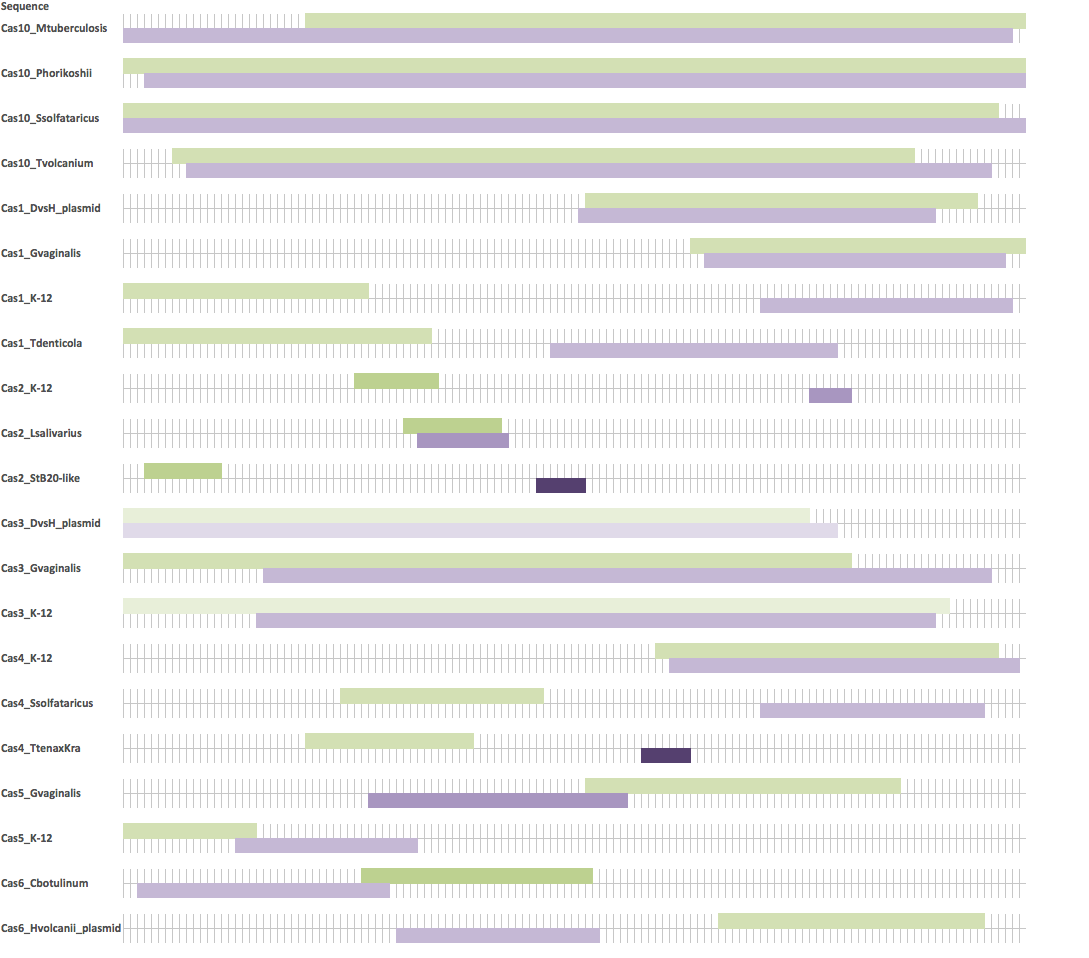
\includegraphics[scale = 0.45]{images/dp_figure1}
      \caption{Pairwise sequence alignment of various \textit{Cas} protein sequences against \textit{s. pyogenes Cas9} protein sequence. Green bars show coverage of semi-global alignment of individual sequence against \textit{s. pyogenes Cas9}. Purple bars show coverage of local alignment of individual sequence against \textit{s. pyogenes Cas9}. Darker color indicates higher average score per base, and therefore higher sequence similarity. Each grey marker represents 10 amino acid residues}
      \label{dp1}
\end{figure}

\begin{figure}[ht]
  \centering
  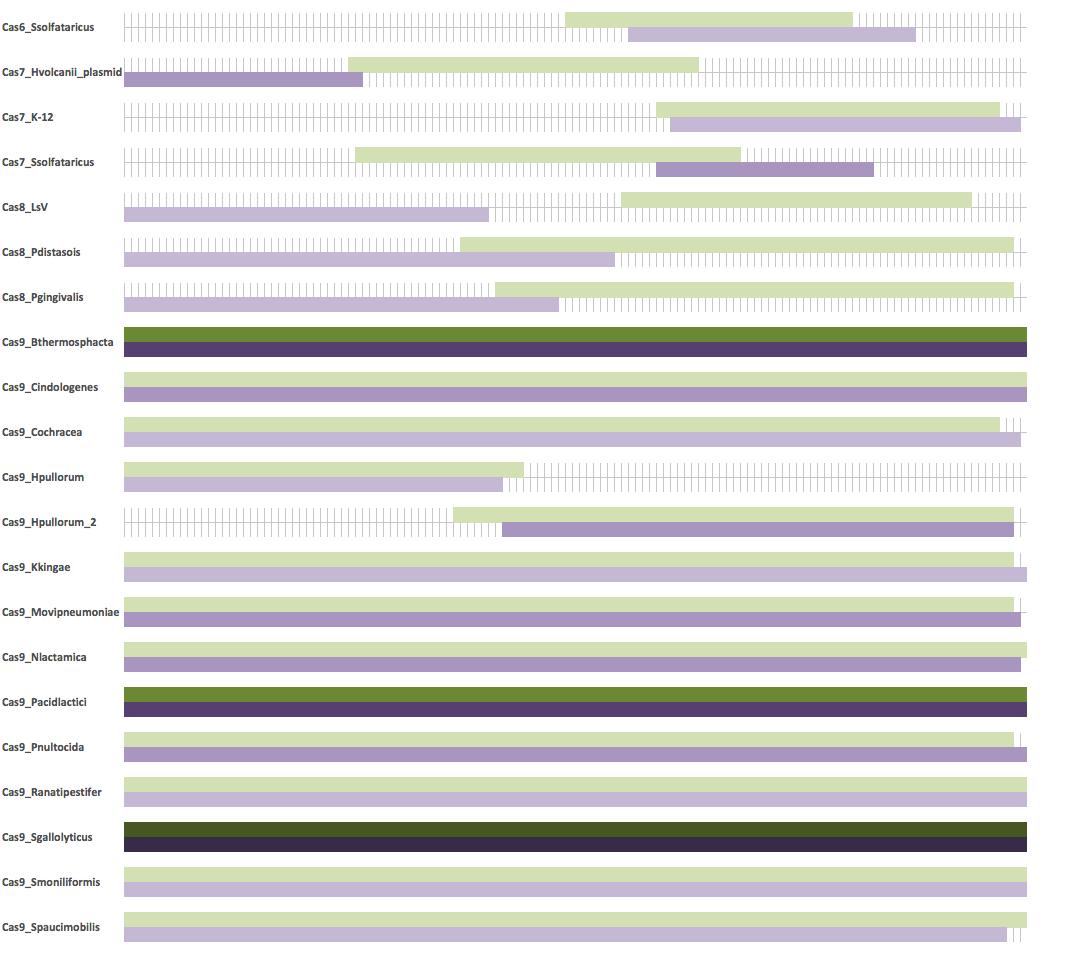
\includegraphics[scale = 0.45]{images/dp_figure2}
      \caption{Pairwise sequence alignment of various \textit{Cas} protein sequences against \textit{s. pyogenes Cas9} protein sequence. Green bars show coverage of semi-global alignment of individual sequence against \textit{s. pyogenes Cas9}. Purple bars show coverage of local alignment of individual sequence against \textit{s. pyogenes Cas9}. Darker color indicates higher average score per base, and therefore higher sequence similarity. Each grey marker represents 10 amino acid residues}
      \label{dp2}
\end{figure}

\subsection{Gibbs Sampling}

f

i

l

l

.

.

.




\subsection{HMM}


f

i

l

l

.

.

.


\section{Conclusion}

.
.
.


\TODO{we need to do this one together}


% trigger a \newpage just before the given reference
% number - used to balance the columns on the last page
% adjust value as needed - may need to be readjusted if
% the document is modified later
%\IEEEtriggeratref{8}
% The "triggered" command can be changed if desired:
%\IEEEtriggercmd{\enlargethispage{-5in}}

% references section

% can use a bibliography generated by BibTeX as a .bbl file
% BibTeX documentation can be easily obtained at:
% http://mirror.ctan.org/biblio/bibtex/contrib/doc/
% The IEEEtran BibTeX style support page is at:
% http://www.michaelshell.org/tex/ieeetran/bibtex/
%\bibliographystyle{IEEEtran}
% argument is your BibTeX string definitions and bibliography database(s)
%\bibliography{IEEEabrv,../bib/paper}
%
% <OR> manually copy in the resultant .bbl file
% set second argument of \begin to the number of references
% (used to reserve space for the reference number labels box)

\TODO{please include any other resources or papers you referenced}

\begin{thebibliography}{1}

\bibitem{IEEEhowto:kopka}
H.~Kopka and P.~W. Daly, \emph{A Guide to \LaTeX}, 3rd~ed.\hskip 1em plus
  0.5em minus 0.4em\relax Harlow, England: Addison-Wesley, 1999.

\bibitem{cas:makarova}
K. S. ~Makarova, et al., \emph{An updated evolutionary classification of CRISPR-Cas systems}  \hskip 1em plus 0.5em minus 0.4em\relax http://dx.doi.org/10.1038/nrmicro3569, 28 September 2015

\bibitem{needlemanwunsch}
Saul B. Needleman, Christian D. Wunsch, \emph{A general method applicable to the search for similarities in the amino acid sequence of two proteins} \hskip 1em plus 0.5em minus 0.4em\relax http://www.sciencedirect.com/science/article/pii/0022283670900574, 28 March 1970

\bibitem{smithwaterman}
Smith, Temple F., Waterman, Michael S., \emph{Identification of Common Molecular Subsequences} \hskip 1em plus 0.5em minus 0.4em\relax Journal of Molecular Biology. 147: 195-197. doi:10.1016/0022-2836(81)90087-5. PMID 7265238., 1981

\bibitem{hmmer}
HMMER 3.1b2 (February 2015); http://hmmer.org/

\end{thebibliography}




\end{document}


